
% ??ds learn about, experiment with and disccuss symplecity?

% The fixed step midpoint method is ``almost symplectic'' for the LLG equation with zero damping, , \ie the property equivalent to Hamiltonian flow for  dissipative systems is conserved up to \order{??ds} \cite{daquino2005} \cite{Austin1993}.

% It is well known that most adaptive schemes are not symplectic\cite[91]{Iserles2009} because they constantly change the ``nearby Hamiltonian'' that is followed by the symplectic integrator.
% Therefore the adaptive IMR is not expected to have the almost-symplectic property discussed in \autoref{??ds}.



\chapter{Application of the adaptive implicit midpoint rule to micromagnetics}
\label{sec:aimr-llg}

In this section we discuss the application of the adaptive implicit midpoint rule to strong form micromagnetics problems (\ie the ODE form and finite difference based methods).
The extension to weak form problems (\ie finite element methods) is discussed in \autoref{sec:nodal-integration}.

\section{Why use the implicit midpoint rule}

The Landau-Lifshitz-Gilbert equation with constant applied field has certain fundamental properties (see \autoref{sec:prop-cont-llg} for a derivation of these properties):
\begin{itemize}
\item Magnetisation length is constant.
\item Energy is dissipated at a rate determined only by the damping constant.
\item Energy is conserved when $\dampc = 0$.
\end{itemize}
In a varying applied field the Zeeman energy may vary independently of damping, which can drive other effects.
However similar energy balance equations can still be derived.

In contrast to most time integrators the implicit midpoint rule conserves the magnetisation length, conserves energy at zero damping in constant applied field and gives highly accurate energy dissipation in linear applied fields\cite{DAquino2005} (see \autoref{sec:prop-imr-llg} for details).
Time integration schemes with conservation properties similar to these are known as geometric integration schemes. 

Since IMR is a single step method there is no dependence on $\dtx{n-1}$ (unlike, for example, BDF2) and so no change in these properties would be expected when going from fixed to varying time step sizes.

We have a number of reasons to believe that such improvements in the accuracy of these properties will translate into an improvement in the accuracy and robustness of the overall solver:
\begin{itemize}
\item Errors in the energy dissipation \cite{Albuquerque2001} and magnetisation length \cite{Chantrell2001} have been successfully used as error estimators for total error.

\item It is well known that geometric integration schemes typically result in much smaller long-timescale error-build-up than schemes that do not preserve such quantities \cite[77]{Iserles2009}.

\item The non-linear modification to the Landau-Lifshitz-Gilbert equation caused by renormalisation of the magnetisation length (as commonly used to maintain correct magnetisation length in non-conservative time integrators) may cause significant changes in the magnetostatic field \cite{Lewis2003}.

\item Renormalisation of the magnetisation modifies the balance between the various energy terms.
  This is similar to the methods that lead to the ``flying ice cube'' problem \cite{Harvey1998} in molecular dynamics.\footnote{In such molecular dynamics the rescaling of particle velocities (to maintain constant temperature despite numerical error accumulation) can result in large amounts of kinetic energy being transferred from the motion of internal degrees of freedom to motion of the centre of mass.}
\end{itemize}

In addition to these conservation properties the following properties make IMR suitable for micromagnetics problems
\begin{itemize}
\item It is second order, which is typically considered a good compromise between speed and accuracy for pdes (higher orders would require expensive high order spatial discretisation to be effective, generally better to just do h-refinement instead).\cite{Matthias}
\item It is A-stable, and so remains efficient for stiff problems such as those arising from the spatial discretisation of PDEs (see \autoref{cha:stiffn-llg-equat}).
\end{itemize}


\section{Geometric properties of the IMR-discretised LLG (strong form)}
\label{sec:prop-imr-llg}

We repeat the procedures used in \autoref{sec:prop-cont-llg} for the discrete form of the Landau-Lifshitz-Gilbert equation that results from the use of the implicit midpoint rule.

As noted in \autoref{sec:extens-impl-odes} IMR is defined by the following substitutions:
\begin{align}
  \label{eq:55}
  \pd{\mv}{t} &\rightarrow \frac{\mv_{n+1} - \mv_n}{\dtn}, \\
  \mv &\rightarrow \frac{\mv_{n+1} + \mv_n}{2}, \\
  t &\rightarrow \frac{t_{n+1} + t_n}{2}.
\end{align}

So the discretised LLG is
\begin{equation}
  \frac{\mv_{n+1} - \mv_n}{\dtn} = - \frac{\mv_{n+1} + \mv_n}{2} \times
  \left(
  \hv \left[\frac{\mv_{n+1} + \mv_n}{2} \right]
  + \happ\left(\frac{t_{n+1} + t_n}{2}\right)
  - \dampc \frac{\mv_{n+1} - \mv_n}{\dtn}
  \right),
  \label{eqn:disc-llg}
\end{equation}
where we have separated the applied field from the rest of the effective field because 1) it is independent of $\mv$ and 2) it is the only field with explicit time dependence.

Intuitively the conservation properties of the IMR discretisation come from the cancellation of cross terms in $\ip{\lop[\mv]}{\dmdt}$ for any symmetrical linear operator $\lop$. More precisely:
\begin{equation}
  \begin{aligned}
    \label{eqn:imr-linop}
    \ip{\lop \left[ \frac{\mv_{n+1} + \mv_n}{2} \right]}{ \frac{\mv_{n+1} - \mv_n}{\dtn} }
    &= \frac{1}{2\dtn} \Big[
      \ip{\mv_{n+1}}{\lop \mv_{n+1}} + \ip{\mv_{n+1}}{\lop \mv_{n}} \\
      & \qquad\qquad - \ip{\mv_{n}}{\lop \mv_{n+1}} - \ip{\mv_{n}}{\lop \mv_{n}}
      \Big] \\
    &= \frac{1}{2\dtn} \Big[
      \ip{\mv_{n+1}}{\lop \mv_{n+1}}
      - \ip{\mv_{n}}{\lop \mv_{n}}
      \Big].
  \end{aligned}
\end{equation}

We can examine the change in magnetisation length similarly to in \autoref{sec:prop-cont-llg}: take the dot product with $\frac{\mv_{n+1} + \mv_n}{2}$ on both sides of~\eqref{eqn:disc-llg} and use~\eqref{eq:dot-cross-id} to get
\begin{equation}
  \frac{\mv_{n+1} + \mv_n}{2} \cdot \frac{\mv_{n+1} - \mv_n}{\dtn} = 0.
\end{equation}
Now using~\eqref{eqn:imr-linop} with $\lop$ the identity operator gives us
\begin{equation}
  \begin{aligned}
    \frac{\ip{\mv_{n+1}}{\mv_{n+1}} - \ip{\mv_n}{\mv_n} }{2 \dtn} &= 0, \\
    \abs{\mv_{n+1}} - \abs{\mv_n} &= 0.
  \end{aligned}
\end{equation}
So the magnetisation length does not change.

Before we can derive energy decay properties of the discretised LLG we need to look at the properties of the effective field when considered as an operator on $\mv$.
We split the effective field into one operator containing the exchange, magnetostatic and magnetocrystalline anisotropy fields and a separate function for the applied field only:
\begin{equation}
  \label{eq:hop}
  \hv(\xv, t)[\mv(\xv)] = \hop [\mv(\xv)] + \happ(\xv, t).
\end{equation}
It can be shown (see \autoref{sec:linear-symm-field-operators}) that $\hop[\mv]$ is a linear symmetric operator on $\mv$ provided that there is no surface anisotropy and that the magnetocrystalline anisotropy is uniaxial (extensions may be possible.. not really checked).
The applied field is not an operator at all so we treat it separately. The energy can be written using this operator (see \autoref{sec:energy-field-relation}) as
\begin{equation}
  \label{eq:energy-hop}
  \e_n = \ehop_{,n} + \eapp_{,n} = - \ip{\mv_n}{\frac{\hop[\mv_n]}{2}} - \ip{\mv_n}{\happ(t_n)}.
\end{equation}
We also expand $\mphapp$ into a midpoint-like form
\begin{equation}
  \mphapp = \frac{\happ(t_{n+1}) + \happ(t_n)}{2} + \order{\dtn^2 \spd{\happ}{t}}.
  \label{eq:happ-midpoint}
\end{equation}
For now we will assume that $\happ$ is linear within each step so that the error term is zero, for details about this see \autoref{sec:non-linear-applied}.

Again in the same manner as the previous section we derive the change in energy of the discrete LLG by taking the $\ltwo$ inner product of equation~\eqref{eqn:disc-llg} with
\begin{equation}
  \mphop + \frac{\happ(t_{n+1}) + \happ(t_n)}{2} - \dampc \mpdmdt,
\end{equation}
resulting in
\begin{equation}
  \begin{aligned}
    &\ltip{\mphop + \frac{\happ(t_{n+1}) + \happ(t_n)}{2}}{\mpdmdt} \\
    & \quad - \dampc \ltip{\mpdmdt}{\mpdmdt} = 0.
    \label{eq:54}
  \end{aligned}
\end{equation}
The $\hop$ term can be simplified by using identity~\eqref{eqn:imr-linop} then written as an energy using equation~\eqref{eq:energy-hop}
\begin{equation}
  \begin{aligned}
    &\frac{1}{2\dtn} \Big[\ip{\mv_{n+1}}{\hop \left[\mv_{n+1} \right]}
      - \ip{\mv_{n}}{ \hop\left[ \mv_{n} \right]} \Big], \\
    &= -\frac{\ehop_{,n+1} - \ehop_{,n}}{\dtn}.
  \end{aligned}
  \label{eq:50}
\end{equation}
Next we examine the $\happ$ term. By adding and subtracting $\happ(t_{n+1}) + \happ(t_n)$ from different parts of the equation, then rearranging and again using equation~\eqref{eq:energy-hop} we obtain
??ds add at least one more step here
\begin{equation}
  \begin{aligned}
    &\frac{ \ip{\happ(t_{n+1})}{\mv_{n+1}} - \ip{\happ(t_n)}{\mv_{n}}}{\dtn}
    + \frac{\ip{\happ(t_{n+1}) -\happ(t_n)}{\mv_{n+1} + \mv_{n}}}{2\dtn}, \\
    &= -\frac{\eapp_{, n+1} - \eapp_{, n}}{\dtn}
    - \ip{\frac{\happ(t_{n+1}) -\happ(t_n)}{\dtn}}{\frac{\mv_{n+1} + \mv_{n}}{2}}.
  \end{aligned}
  \label{eq:52}
\end{equation}
Finally we insert the results of equations~\eqref{eq:50} and \eqref{eq:52} into \eqref{eq:54} to find
\begin{equation}
  \frac{\e_{n+1} - \e_n}{\dtn}
  = -\dampc \ltip{\mpdmdt}{\mpdmdt}
  - \ip{\frac{\happ(t_{n+1}) -\happ(t_n)}{\dtn}}{\frac{\mv_{n+1} + \mv_{n}}{2}},
\label{eqn:imr-llg-energy}
\end{equation}
which is exactly the midpoint discretisation of the continuous energy balance equation~\eqref{eq:energy-decay}.

Note that nothing in the above derivations depends in previous step sizes, hence these properties should hold regardless of any variations in step size (\ie in an adaptive time integrator).

??ds draw commutation diagram
??ds physical interpretation in terms of energy?
??ds comparison for TR? BDF2?


\section{Limitations and alternatives}

\subsection{Non-linear applied fields}
\label{sec:non-linear-applied}

In the previous section we assumed that the applied field, $\happ$, is linear (within each step).
We now examine what happens when $\happ$ is not linear.

First when $\happ$ is piecewise linear, for example instantaneously switching on a field at a certain point in time.
In this case we can avoid any problems by selecting time steps such that each non-linear change happens exactly at the start/end of a step.
As long as the time between non-linear changes in field is long compared to the time scale of the dynamics this will have no effect on the efficiency.

In the case when the field is genuinely non-linear there is an additional error term added to the energy balance equation~\eqref{eqn:imr-llg-energy}:
\begin{equation}
  err =
\end{equation}


\subsection{Solvers}

It should be noted that the above properties are only true up to the accuracy with which we solve the LLG. Since the LLG is non-linear this is typically the Newton tolerance.

Additionally the derivation assume that all fields are calculated at the midpoint without any additional approximations, \ie that we are using a fully implicit method.
In contrast to this, many existing FEM/BEM models use an explicit approximation to the magnetostatic field.
Unfortunately in this case the energy properties will be lost (or at least reduced in effectiveness) due to the replacement of $\hop \left[ \mpm \right]$ by different approximation.
However the magnetisation length property will be retained because this only relies on $\mv$ itself being calculated implicitly.

Efficient, fully-implicit solvers, as required to realise the full potential of the implicit midpoint rule, are certainly possible: one example was implemented by d'Aquino \etal.\cite{DAquino2005}


\subsection{Alternative conserving time integration methods in micromagnetics}

??ds move to later, after FEM section

??ds spherical polars:
- singular coordinate system!!

The conservation of magnetisation length by IMR does not require a fully implicit calculation as demonstrated by Spargo \etal\cite{Spargo2003a}.
Hence the our adaptive IMR scheme could be also be useful in a semi-implicit magnetisation-length-conserving solver.

??ds Cayley transforms

??ds Linearised + projection version by analyst guys

- Decent speed increase (one lin solve vs two)
- But only first order! (can be extended to second order but then non-linear again, no improvement over IMR)
- fem only


\subsection{Alternative time adaptivity methods in micromagnetics}
\label{sec:altern-time-adapt}

In cases where the damping is not exact the effective damping can be used as an error estimator, as proposed by Albuquerque \etal\cite{Albuquerque2001}
??ds The disadvantage of this method (aside from the obvious requirement that the damping be inexact) is that, depending on the discretisation used, the error estimator may be unable to distinguish between insufficient space refinement and insufficient time refinement.
In particular this is the case when the solution is not completely divided into separate effective field calculations and pointwise time integration, such as in a typical Galerkin finite element model.

Rigorous time error estimates for the LLG with limited effective field terms with a certain discretisation method were proven and used to perform adaptive refinement of midpoint method time steps by Banas.\cite{Banas-thesis}
??ds do these work, why does no one use them?
By comparison our adaptive method is much more general in that it can be applied to any differential equation and any discretisation scheme which uses the method of lines for time.
It is also simpler to implement (requiring only an additional explicit time step, which can easily be handled by existing ODE solver packages) and easy to understand.




\section{Numerical Experiments}
\label{sec:imr-ode-llg-numer-exper}

In this section we present numerical experiments with adaptive IMR on a simple LLG problem.
We show that the adaptive midpoint method retains the conservation properties of the fixed step midpoint method and that the adaptivity is effective when applied to the LLG.
Experiments with more complex examples are shown in \autoref{sec:numer-exper} and \autoref{cha:numer-experiments}.

To avoid introducing spatial discretisation issues we choose an example problem that can be modelled using only an ODE: the reversal of a ``small'' spherical particle under spatially-uniform applied field.
With this geometry and with uniform initial magnetisation the magnetostatic field can be analytically shown to be $\hms = -\mv/3$ throughout the domain \cite[112]{Aharoni1996}.
This means that the magnetisation remains uniform for sufficiently small spheres such that the increase in exchange energy is larger than the decrease in magnetostatic energy that could be gained by a non-uniform state.

In this case the Landau-Lifshitz form of the Landau-Lifshitz-Gilbert equation \eqref{eqn:nd-llg-full} reduces to
\begin{equation}
  \begin{aligned}
    (1 + \dampc^2) \dmdt &= - \mv \times \hv - \dampc \mv \times \bigs{\mv \times \hv}, \\
    \hv &= \happ + \kone (\mv \cdot \ev) \ev.
    \label{eqn:nd-ode-llg}
  \end{aligned}
\end{equation}

To simplify the problem even further we choose $\kone = 0$ and $\happ(t) = [0, 0, -H]$.
In this case an exact solution is available for the time taken for $\mv$ to reach a given angle to the $z$-axis, and for the amount of precession that will take place in that time.\footnote{Actually the solution can be easily extended to $\kone \neq 0$ with $\ev = \unitz$ and any $z$-aligned ellipsoid of rotation \cite{Mallinson2000}.}
The exact solution is best expressed in spherical polar notation:
\begin{equation}
  \begin{aligned}
    \theta &= \cos^{-1}(m_z/1),\\
    \phi &= \tan^{-1}(m_y/m_x),
  \end{aligned}
\end{equation}
so $\theta$ is the angle between $\mv$ and the $+z$-direction.
We use the usual notation that $\theta_n$ is the approximation to the exact solution at time $t_n$.
The time for a reversal from the initial value $\theta_0$ to $\theta$ is given by
\begin{equation}
  \tau(\theta) = t_0 + \frac{\dampc^2 +1}{H \dampc}
  \ln \bigb{ \frac{\tan(\theta/2)}{\tan(\theta_0/2)} }.
\end{equation}
The azimuthal angle precessed through during this switching is
\begin{equation}
  \varphi(\theta) = \phi_0 +  \frac{-1}{\dampc} \ln \bigb{ \frac{\tan(\theta/2)}{\tan(\theta_0/2)} }.
\end{equation}

Given this we choose as the error norm
\begin{equation}
  e = \abs{\tau(\theta_n) - t_n},
\end{equation}
\ie the absolute error in the switching time, because the switching of the magnetisation is typically more important than the precession.

We choose parameters $H = 1.1$ (??ds why?) and $\dampc = 0.01$ (roughly the physically relevant value). 
The initial magnetisation is just off the $z$-axis in order to avoid a singularity in the reversal time when $\theta_1 = 0$, more precisely $\mv_0 = (0.01, 0.0, 1.0)/\sqrt{1.0001}$. 
The maximum time is set to 1000 units for all simulations (enough for the magnetisation to fully switch with this damping constant).


In the experiments below the LL form \eqref{eq:ll-nd-llglike} of the LLG is used for ease of implementation.
Linearisation is carried out using the Newton-Raphson method, the $3 \times 3$ Jacobian is calculated analytically and inverted using a direct solve.
Unless otherwise specified the Newton tolerance is $\newtontol = 10^{-12}$, the adaptive integrator tolerance is $\toltt = 10^{-4}$ and the initial time step is $\dtinitial = 10^{-3}$ (small enough to allow the adaptive algorithm to naturally increase to the required value).

The Newton residual is
\begin{equation}
  \rv = (1 + \dampc^2) \dmdt + \skewm{\mv} \cdot \hv + \dampc \skewm{\mv}\skewm{\mv} \cdot \hv. \\
\end{equation}
The corresponding Jacobian can be easily derived using the methods discussed in \autoref{sec:llg-jacobian}, it is:
\begin{equation}
  J = (1 + \dampc^2) J_{ts} \Idm_3 - \skewm{\hv} - \dampc \skewm{ \mv \times \hv }
  - \dampc \skewm{\mv} \skewm{\hv}.
\end{equation}

This experiment allows us to check the conservation properties of IMR, to compare the accuracy of the solution over different time integrators, and to check that the time step selected is properly increased as the solution is damped out.

The behaviour of the magnetisation and the time step selection is shown in \autoref{fig:imr-llg-ode}.
Time step selection working as expected: large at the start, decreases as switching occurs, then grows again. 
The many small peaks in time step are due to the periodicity of the precession ??ds zoomed in view?

\begin{figure}[tbp]
  \centering
  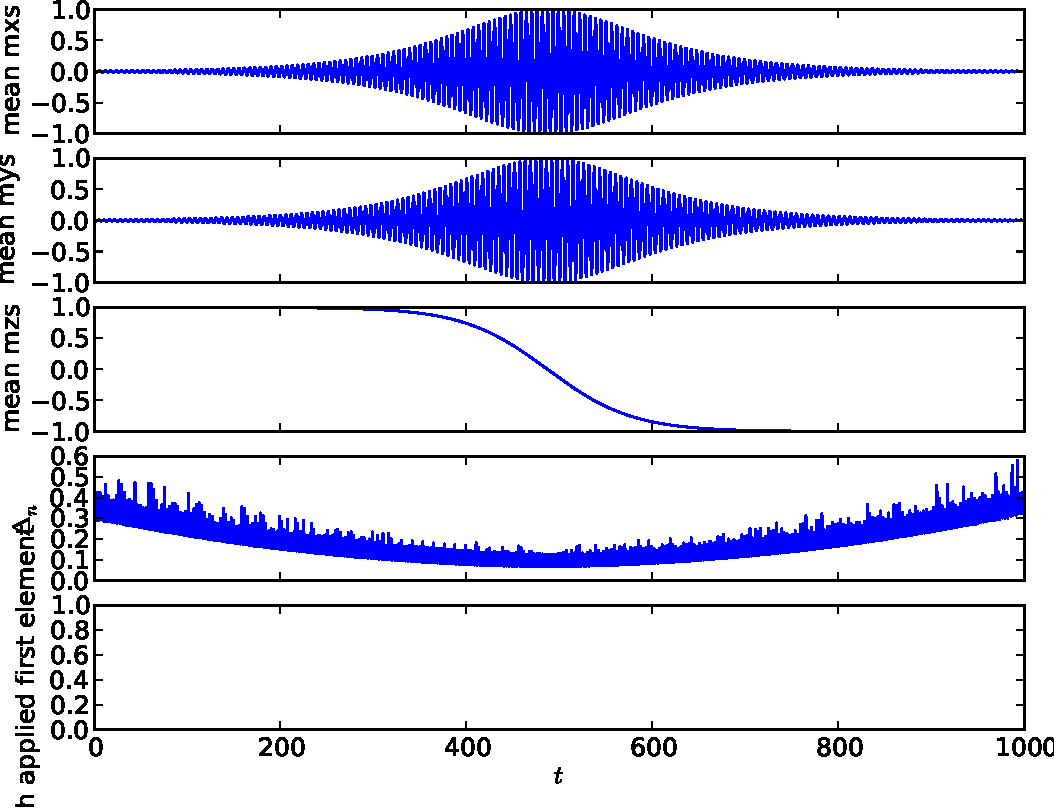
\includegraphics[width=0.8\textwidth]{plots/aimr-sphere-relax/meanmxsvs-meanmysvs-meanmzsvs-dtsvs-happliedfirstelementvstimes.pdf}
  \caption{Plot of $\mv$ and $\dtn$ over time for the relaxing nano-sphere problem solved by adaptive IMR.}
  \label{fig:imr-llg-ode}
\end{figure}

\subsection{Conservation properties}

The conservation of the magnetisation length is shown in \autoref{fig:ml-aimr-ode}.
For comparison the same calculation using BDF2 and TR results in magnetisation length errors of order $10^{-3}$ and $10^{-4}$ respectively.
To show that this conservation property is not dependent on $\dampc$, $\toltt$ or $\dtn$ we ran the experiment for each damping of $\dampc= 1, 0.1, 0.01$ with fixed steps of $\dtn=0.1, 0.05, 0.01, 0.005$ and adaptive step with $\toltt =10^{-2}, 10^{-3}, 10^{-4}, 10^{-5}, 10^{-6}$. 
The maximum error in magnetisation length was $1.07\E{-10}$, easily within the range of Newton error build-up.
% ./parameter-sweep.py -p imr_ode_llg -p aimr_ode_llg --clean && parse.py --print-data max-max-ml -d /mnt/moredata/optoomph/user_drivers/micromagnetics/experiments/parameter_sweeps/aimr_ode_llg -f "('-ts', 'imr')" -d /mnt/moredata/optoomph/user_drivers/micromagnetics/experiments/parameter_sweeps/imr_ode_llg

\begin{figure}[tbp]
  \centering
  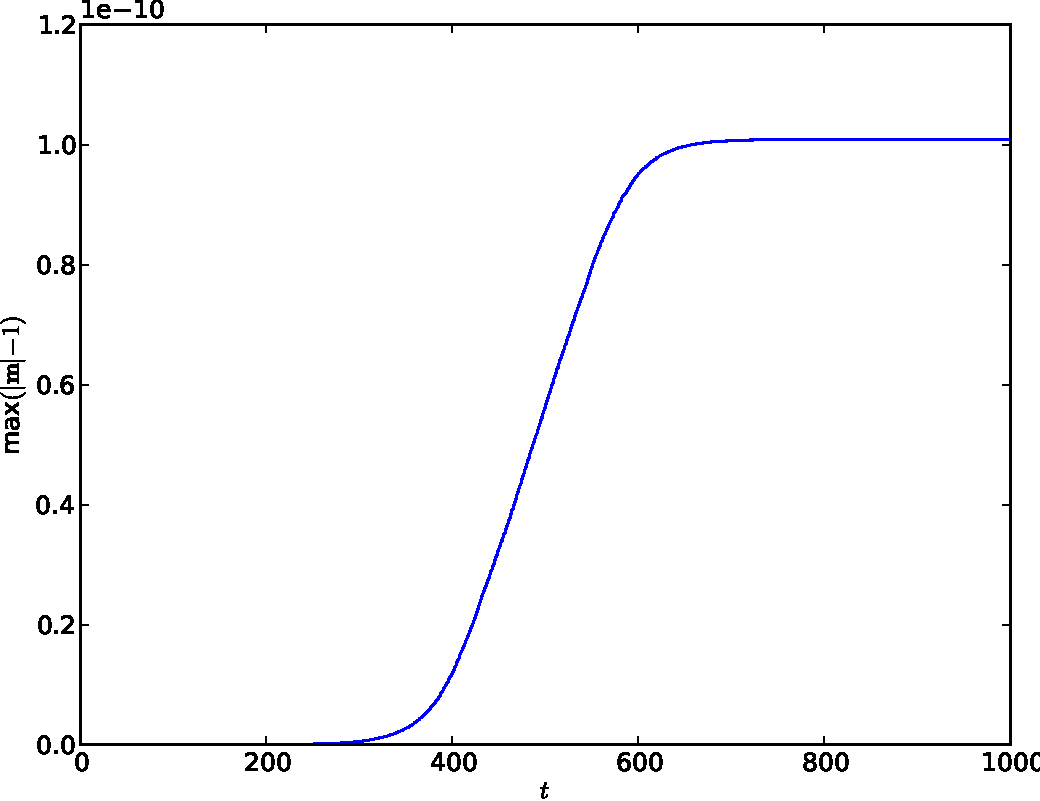
\includegraphics[width=0.8\textwidth]{plots/aimr-sphere-relax/mlengtherrormaxesvstimes.pdf}
  \caption{Magnetisation length error, $\abs{\abs{\mv} -1}$, over time for the relaxing nano-sphere problem solved by adaptive IMR.}
  \label{fig:ml-aimr-ode}
\end{figure}

The effective damping ??ds shown in \autoref{fig:aimr-llg-ode-energy}.

\begin{figure}[tbp]
  \centering
  
\includegraphics[width=0.8\textwidth]{images/placeholder}
  \caption{??ds plot of energy conservation.}
  \label{fig:aimr-llg-ode-energy}
\end{figure}


\subsection{Comparison with other methods}


\begin{figure}[tbp]
  \centering
  
\includegraphics[width=0.8\textwidth]{images/placeholder}
  \caption{??ds convergence plot of accuracy--constant step and adaptive step}
  \label{fig:imr-llg-ode-accury}
\end{figure}


??ds plot of bdf2 failing utterly?


For comparison in \autoref{fig:bdf2-llg-ode} we show a plot of the solution calculated using the same parameters but using the BDF2 method.
The accuracy of the switching time is completely terrible, this is probably due to L-stability.
TR accuracy is good, but requires renormalisation.


\section{Conclusions}

??ds


%%% Local Variables:
%%% mode: latex
%%% TeX-master: "./main"
%%% End:
